% AER-Article.tex for AEA last revised 22 June 2011
\documentclass[AER]{AEA}

% The mathtime package uses a Times font instead of Computer Modern.
% Uncomment the line below if you wish to use the mathtime package:
%\usepackage[cmbold]{mathtime}
% Note that miktex, by default, configures the mathtime package to use commercial fonts
% which you may not have. If you would like to use mathtime but you are seeing error
% messages about missing fonts (mtex.pfb, mtsy.pfb, or rmtmi.pfb) then please see
% the technical support document at http://www.aeaweb.org/templates/technical_support.pdf
% for instructions on fixing this problem.

% Note: you may use either harvard or natbib (but not both) to provide a wider
% variety of citation commands than latex supports natively. See below.

% Uncomment the next line to use the natbib package with bibtex
\usepackage{natbib}

% Uncomment the next line to use the harvard package with bibtex
%\usepackage[abbr]{harvard}

% This command determines the leading (vertical space between lines) in draft mode
% with 1.5 corresponding to "double" spacing.
\draftSpacing{1.5}


% tightlist command for lists without linebreak
\providecommand{\tightlist}{%
  \setlength{\itemsep}{0pt}\setlength{\parskip}{0pt}}



\usepackage{graphicx}
\usepackage{booktabs}

\usepackage{hyperref}

\begin{document}


\title{Global \(CO_{2}\) Emissions 1995 and Pressent}
\shortTitle{What Keeling missed all these years}
% \author{Author1 and Author2\thanks{Surname1: affiliation1, address1, email1.
% Surname2: affiliation2, address2, email2. Acknowledgements}}


\author{
  Yuna Kim, Jinsoo Chung, Priya Reddy, Jocelyn Thai\thanks{
  : , \href{mailto:}{}.
  The authors would like to thank their instructors from MIDS 271.
}
}

\date{\today}
\pubMonth{03}
\pubYear{2023}
\pubVolume{0}
\pubIssue{0}
\JEL{}
\Keywords{Replication, Modern Science}

\begin{abstract}
Global average temperatures have increased by more than 1℃ since
pre-industrial time and the increase of carbon emission has played a key
role in the global warming. Human emissions of carbon dioxide and other
greenhouse gases are a primary driver of climate change.The rapid
warming itself can have significant impacts on climate and natural
systems across the world and human's greed for industrialization may
have caused it.
\end{abstract}


\maketitle

Understanding a changing climate, and what it means for the earth's
inhabitants is of growing interest to the scientific and policy
community. Although, at this point in 1997 it is not entirely clear what
the consequences of this growing awareness will be, in this report we
present likely outcomes under ``business-as-usual'' scenarios. In doing
so, our hope, is to establish a series of possible futures, and, as
evidence, technology, and policy develop over the coming decades, that
we can weigh the impacts that carbon-emission reduction efforts might
take.

\hypertarget{background}{%
\section{Background}\label{background}}

\hypertarget{carbon-emissions}{%
\subsection{Carbon Emissions}\label{carbon-emissions}}

We want to understand if atmospheric CO2 levels increased since 1997 and
if we anticipate that this trend will continue. High CO2 levels have
been shown to negatively play into climate change. The increase in
atmospheric CO2 has cascading effects from global warming to ocean
acidification. Due to this, we may notice food supply chain disruptions,
natural disasters of increasing intensity, and habitat disruption of all
ecosystems and the animal species living there. In an economical sense,
understanding these patterns is important so we can prepare for any
shifts and uncertainities in supply chains that might arise for these
new climate patterns. In total understanding the patterns in atmospheric
CO2 concentrations is important both so that we can mitigate the
existing effects of this increase and prevent continuing upwards trends
in CO2. In addition if our findings are significant, this could persuade
other governmental organizations to increase their CO2 monitoring
efforts.

\hypertarget{historical-trends-in-atmospheric-carbon}{%
\subsection{Historical Trends in Atmospheric
Carbon}\label{historical-trends-in-atmospheric-carbon}}

In 1958 Keeling began continuous monitoring of atmospheric carbon
dioxide concentrations from the Mauna Loa Observatory in Hawaii and soon
observed a trend increase carbon dioxide levels in addition to the
seasonal cycle. He was able to attribute this trend increase to growth
in global rates of fossil fuel combustion. This trend has continued to
the present, and is known as the ``Keeling Curve.''

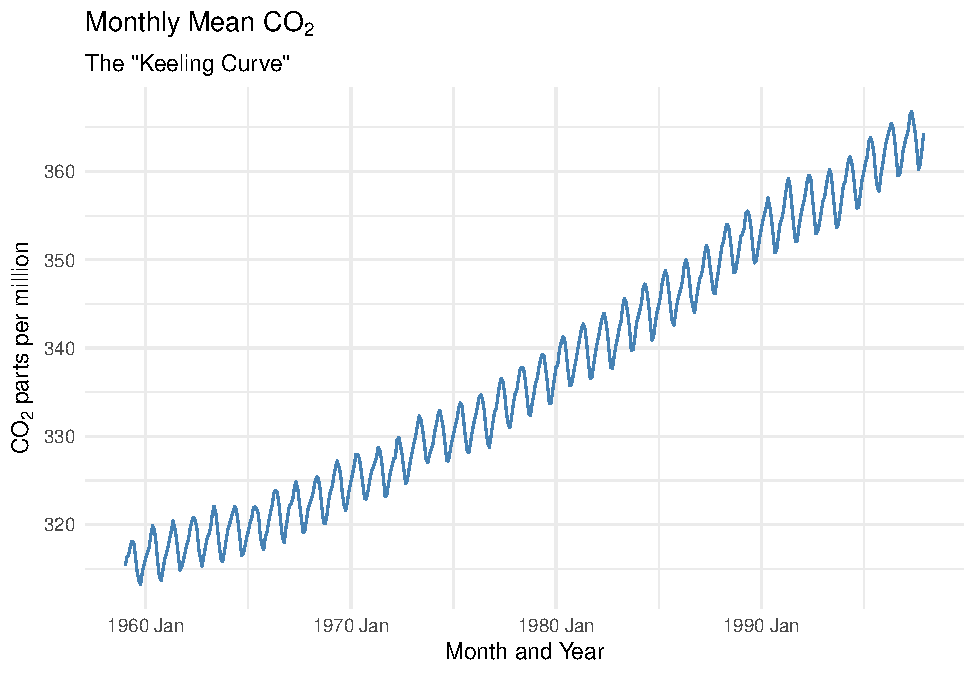
\includegraphics{Lab2_Group_report_files/figure-latex/plot the keeling curve-1.pdf}

\hypertarget{models-and-forecasts}{%
\section{Models and Forecasts}\label{models-and-forecasts}}

In this section, we present evaluate two classes models the linear model
and the ARIMA model to assess which time series model is most
appropriate to use.

\hypertarget{data-eda}{%
\subsection{Data EDA}\label{data-eda}}

This data measures the mean atmospheric CO2 concentration in Mauna Loa
Observatory in Hawaii. The data ranges from 313 parts per million by
volume (ppmv) in March 1958 to 406ppmv in November 2018. The data was
normalized to remove any influence from local contamination. Carbon
dioxide measurements at the Mauna Loa Observatory in Hawaii are made
with a type of infrared spectrophotometer, now known as a nondispersive
infrared sensor, that is calibrated using World Meteorological
Organization standards.

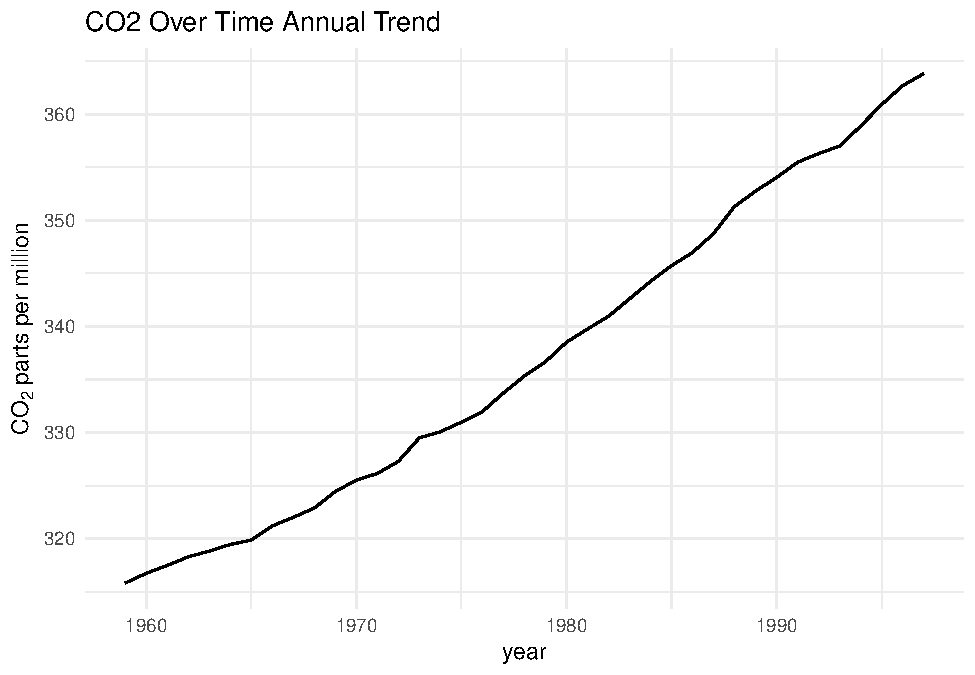
\includegraphics{Lab2_Group_report_files/figure-latex/unnamed-chunk-3-1.pdf}

\begin{verbatim}
## Warning: The dot-dot notation (`..count..`) was deprecated in ggplot2 3.4.0.
## i Please use `after_stat(count)` instead.
\end{verbatim}

\begin{verbatim}
## `stat_bin()` using `bins = 30`. Pick better value with `binwidth`.
\end{verbatim}

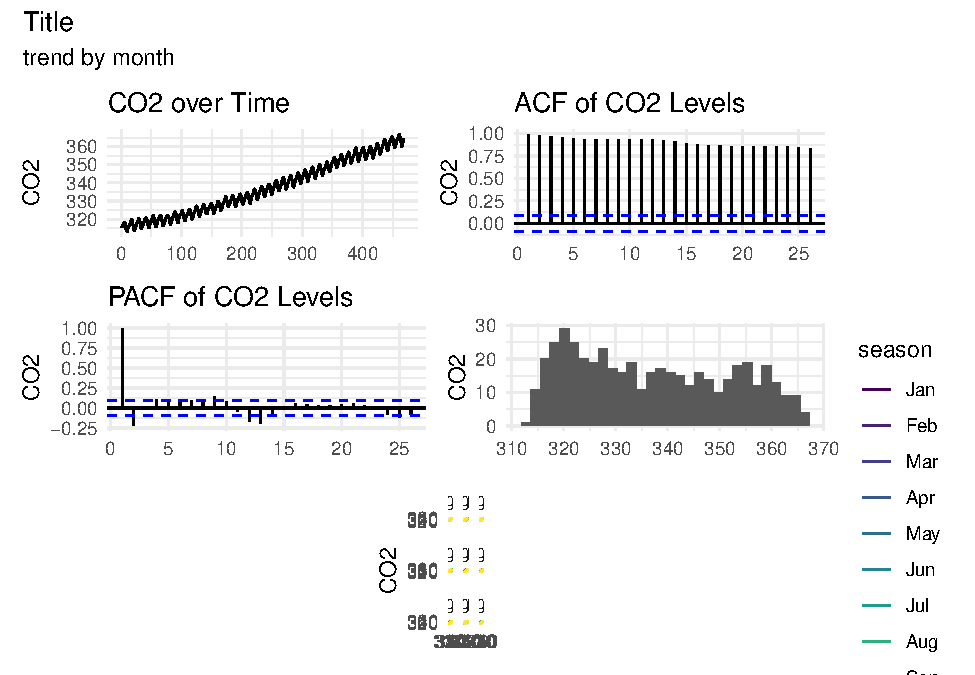
\includegraphics{Lab2_Group_report_files/figure-latex/EDA -1.pdf}

Observations: - Time Series: From the CO2 Over Time plot, there is an
obvious trend of increasing levels throughout time, and we can some
regular oscillations which could mean there is seasonality in the data.
- ACF: There's a gradual decay in the ACF values over the lags, perhaps
indicating there is a trend in the data. - PACF: PACF cuts off to zero
after lag 2 and stays that way. However, at lags 12 and 13, the values
become significant again. This suggests that although the model exhibits
AR model-like behavior, there's some deviances in the data. -
Distribution:

\begin{quote}
Observations: - Time Series: From the yearly CO2 Over Time plot, there
is an obvious trend of increasing levels throughout time, but we can see
that there is no seasonality now. This points to the period of the
seasonal trend being a year. - ACF: There's a gradual decay in the ACF
values over the lags, indicating there is a still a trend in the data.
\end{quote}

\hypertarget{linear-models}{%
\subsection{Linear Models}\label{linear-models}}

\hypertarget{time-series-decompotision}{%
\subsubsection{Time series
decompotision}\label{time-series-decompotision}}

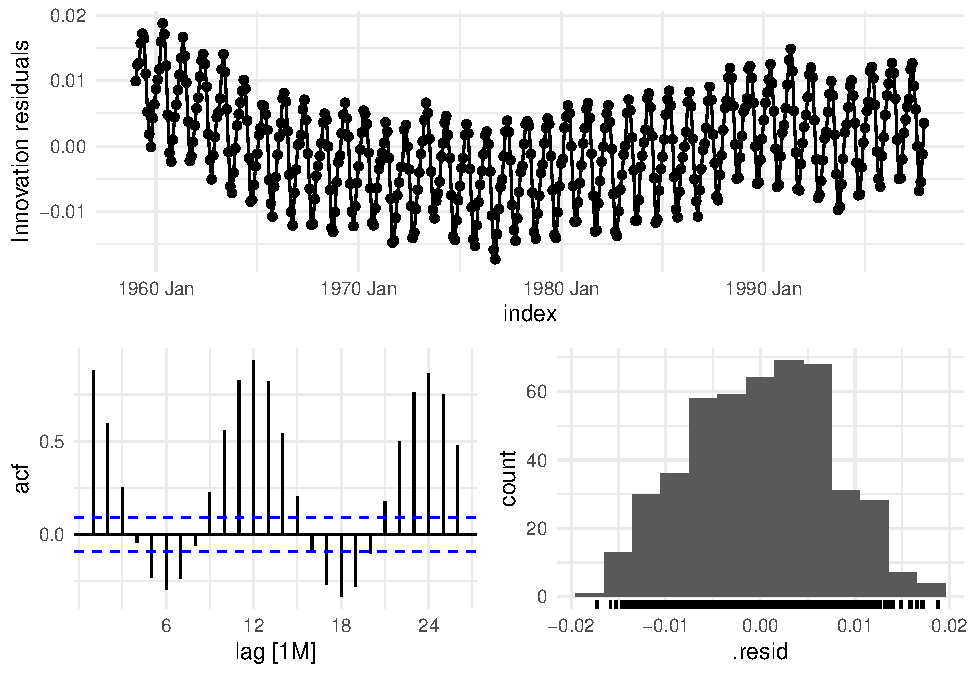
\includegraphics{Lab2_Group_report_files/figure-latex/unnamed-chunk-4-1.pdf}

To fit linear time trend model to the \texttt{co2} series we will
compare a regular time trend linear model to a quadratic time trend
model. We will also fit a polynomial time trend model that incorporates
seasonal dummy variables, and use this model to generate forecasts to
the year 2020.

To begin, we fit a model of the form:

\begin{equation}
\label{eq:one}
\text{CO}_{2} = \phi_{0} + \phi_{1} + \epsilon_{eit}
\end{equation}

\begin{verbatim}
## 
## ==================================================================================================================================
##                                                                  Dependent variable:                                              
##                     --------------------------------------------------------------------------------------------------------------
##                                                                          co2                                                      
##                                 (1)                         (2)                        (3)                         (4)            
## ----------------------------------------------------------------------------------------------------------------------------------
## time(co2)                0.109*** (0.001)            0.067*** (0.003)            0.109*** (0.001)           0.032*** (0.004)      
## I(time(co2)2)                                       0.0001*** (0.00001)                                    0.0003*** (0.00002)    
## I(time(co2)3)                                                                                             -0.00000*** (0.00000)   
## spring                                                                           5.110*** (0.244)           5.070*** (0.136)      
## winter                                                                           2.690*** (0.244)           2.670*** (0.136)      
## summer                                                                           3.440*** (0.244)           3.420*** (0.136)      
## fall                                                                                                                              
## Constant                312.000*** (0.242)          315.000*** (0.304)          309.000*** (0.230)         313.000*** (0.213)     
## ----------------------------------------------------------------------------------------------------------------------------------
## Observations                    468                         468                        468                         468            
## R2                             0.969                       0.979                      0.985                       0.995           
## Adjusted R2                    0.969                       0.979                      0.985                       0.995           
## Residual Std. Error      2.620 (df = 466)            2.180 (df = 465)            1.860 (df = 463)           1.040 (df = 461)      
## F Statistic         14,795.000*** (df = 1; 466) 10,750.000*** (df = 2; 465) 7,419.000*** (df = 4; 463) 15,983.000*** (df = 6; 461)
## ==================================================================================================================================
## Note:                                                                                                  *p<0.1; **p<0.05; ***p<0.01
\end{verbatim}

\begin{verbatim}
## `geom_smooth()` using method = 'loess' and formula = 'y ~ x'
## `geom_smooth()` using method = 'loess' and formula = 'y ~ x'
## `geom_smooth()` using method = 'loess' and formula = 'y ~ x'
## `geom_smooth()` using method = 'loess' and formula = 'y ~ x'
\end{verbatim}

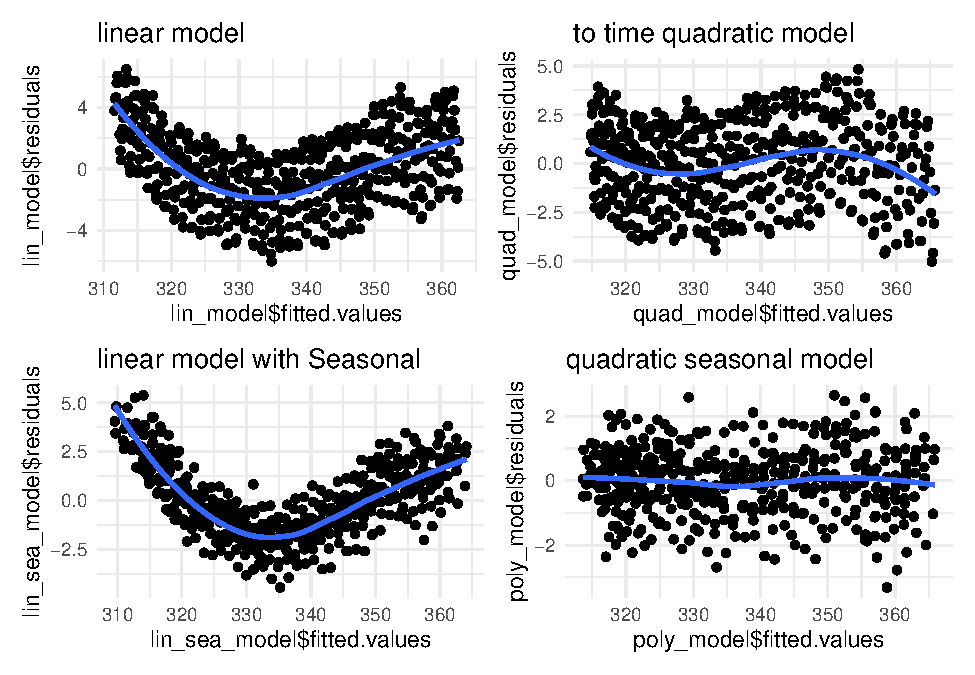
\includegraphics{Lab2_Group_report_files/figure-latex/unnamed-chunk-7-1.pdf}

\hypertarget{model-forcast}{%
\subsection{Model Forcast}\label{model-forcast}}

\begin{verbatim}
## Series: co2 
## Model: TSLM 
## 
## Residuals:
##    Min     1Q Median     3Q    Max 
##  -5.02  -1.71   0.21   1.80   4.83 
## 
## Coefficients:
##              Estimate Std. Error t value Pr(>|t|)    
## (Intercept)  3.15e+02   3.04e-01  1035.7   <2e-16 ***
## trend()      6.74e-02   2.99e-03    22.5   <2e-16 ***
## I(trend()^2) 8.86e-05   6.18e-06    14.3   <2e-16 ***
## ---
## Signif. codes:  0 '***' 0.001 '**' 0.01 '*' 0.05 '.' 0.1 ' ' 1
## 
## Residual standard error: 2.18 on 465 degrees of freedom
## Multiple R-squared: 0.979,   Adjusted R-squared: 0.979
## F-statistic: 1.07e+04 on 2 and 465 DF, p-value: <2e-16
\end{verbatim}

\begin{verbatim}
## # A tibble: 1 x 3
##   .model      lb_stat lb_pvalue
##   <chr>         <dbl>     <dbl>
## 1 trend_model   3838.         0
\end{verbatim}

\begin{verbatim}
## # A tibble: 1 x 5
##   adj_r_squared    CV   AIC  AICc   BIC
##           <dbl> <dbl> <dbl> <dbl> <dbl>
## 1         0.979  4.79  735.  735.  752.
\end{verbatim}

\hypertarget{arima-models}{%
\subsection{ARIMA Models}\label{arima-models}}

Sure we also fit some ARIMA models. And talk about them.

\begin{verbatim}
## <lst_mdl[1]>
## [1] <ARIMA(2,1,4)>
\end{verbatim}

\begin{verbatim}
## # A tibble: 6 x 6
##   .model   term  estimate std.error statistic   p.value
##   <chr>    <chr>    <dbl>     <dbl>     <dbl>     <dbl>
## 1 ts.model ar1     1.69      0.0141   120.    0        
## 2 ts.model ar2    -0.952     0.0142   -67.2   3.61e-242
## 3 ts.model ma1    -1.26      0.0448   -28.1   2.63e-102
## 4 ts.model ma2     0.111     0.0778     1.43  1.53e-  1
## 5 ts.model ma3     0.0703    0.0792     0.887 3.75e-  1
## 6 ts.model ma4     0.266     0.0464     5.72  1.90e-  8
\end{verbatim}


\includegraphics{Lab2_Group_report_files/figure-latex/unnamed-chunk-10-1.pdf}

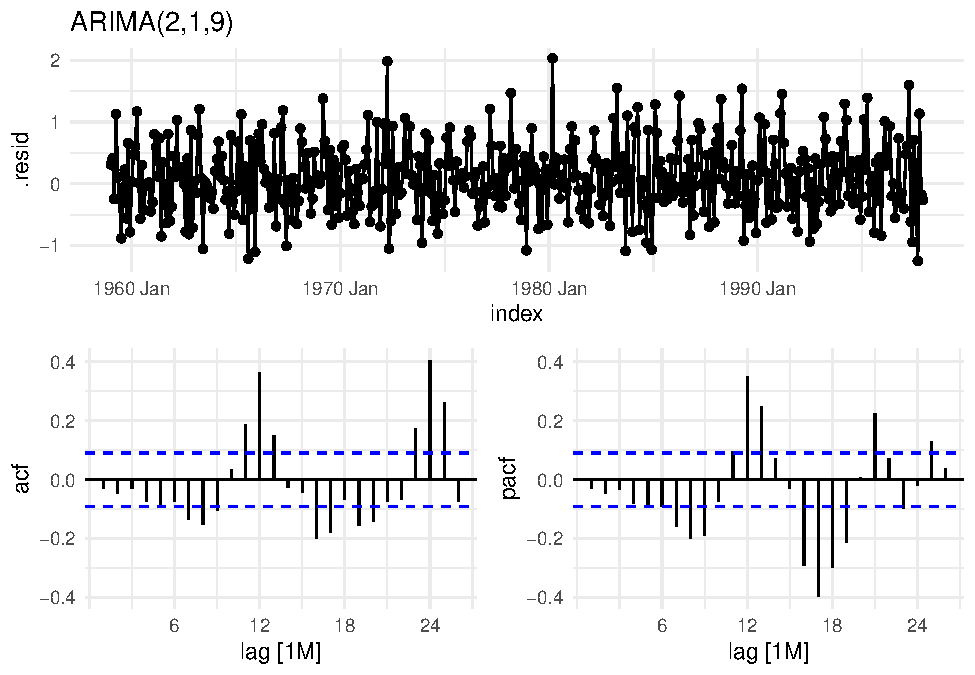
\includegraphics{Lab2_Group_report_files/figure-latex/unnamed-chunk-11-1.pdf}

\hypertarget{forecasts}{%
\subsection{Forecasts}\label{forecasts}}

\hypertarget{report-from-the-point-of-view-of-the-present}{%
\section{Report from the Point of View of the
Present}\label{report-from-the-point-of-view-of-the-present}}

One of the very interesting features of Keeling and colleagues' research
is that they were able to evaluate, and re-evaluate the data as new
series of measurements were released.

\hypertarget{introduction}{%
\subsection{Introduction}\label{introduction}}

In this introduction, you can assume that your reader will have
\textbf{just} read your 1997 report. In this introduction, \textbf{very}
briefly pose the question that you are evaluating, and describe what (if
anything) has changed in the data generating process between 1997 and
the present.

\hypertarget{points-task-1b-create-a-modern-data-pipeline-for-mona-loa-co2-data.}{%
\subsection{(3 points) Task 1b: Create a modern data pipeline for Mona
Loa CO2
data.}\label{points-task-1b-create-a-modern-data-pipeline-for-mona-loa-co2-data.}}

The most current data is provided by the United States' National Oceanic
and Atmospheric Administration, on a data page
{[}\href{https://gml.noaa.gov/ccgg/trends/data.html}{here}{]}. Gather
the most recent weekly data from this page. (A group that is interested
in even more data management might choose to work with the
\href{https://gml.noaa.gov/aftp/data/trace_gases/co2/in-situ/surface/mlo/co2_mlo_surface-insitu_1_ccgg_HourlyData.txt}{hourly
data}.)

Create a data pipeline that starts by reading from the appropriate URL,
and ends by saving an object called \texttt{co2\_present} that is a
suitable time series object.

Conduct the same EDA on this data. Describe how the Keeling Curve
evolved from 1997 to the present, noting where the series seems to be
following similar trends to the series that you ``evaluated in 1997''
and where the series seems to be following different trends. This EDA
can use the same, or very similar tools and views as you provided in
your 1997 report.

\begin{verbatim}
## # A tibble: 6 x 11
##    year month   day decimal average ndays X1.year.ago X10.years.ago increase.s~1
##   <int> <int> <int>   <dbl>   <dbl> <int>       <dbl>         <dbl>        <dbl>
## 1  1997     1     5   1997.    363.     7        362.          349.         83.1
## 2  1997     1    12   1997.    363.     7        362.          349.         83.0
## 3  1997     1    19   1997.    364.     7        362.          349.         83.3
## 4  1997     1    26   1997.    363.     7        363.          349.         82.9
## 5  1997     2     2   1997.    364.     7        363.          349.         83.1
## 6  1997     2     9   1997.    364.     7        363.          348.         83.7
## # ... with 2 more variables: time_index <dttm>, month_index <mth>, and
## #   abbreviated variable name 1: increase.since.1800
\end{verbatim}

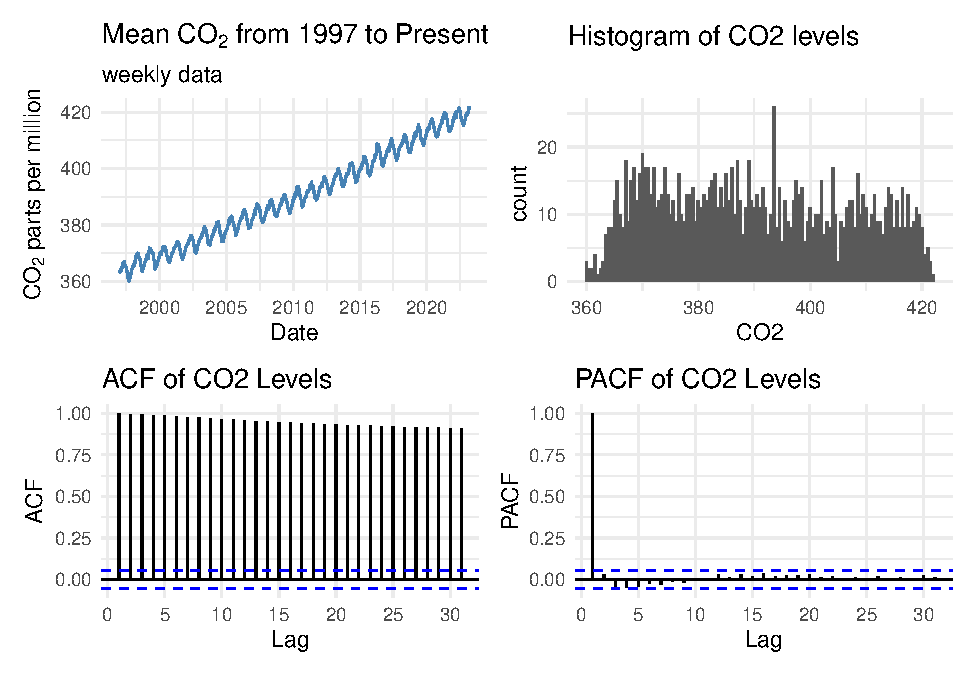
\includegraphics{Lab2_Group_report_files/figure-latex/unnamed-chunk-13-1.pdf}

\hypertarget{point-task-2b-compare-linear-model-forecasts-against-realized-co2}{%
\subsection{(1 point) Task 2b: Compare linear model forecasts against
realized
CO2}\label{point-task-2b-compare-linear-model-forecasts-against-realized-co2}}

Descriptively compare realized atmospheric CO2 levels to those predicted
by your forecast from a linear time model in 1997 (i.e.~``Task 2a'').
(You do not need to run any formal tests for this task.)

\hypertarget{point-task-3b-compare-arima-models-forecasts-against-realized-co2}{%
\subsection{(1 point) Task 3b: Compare ARIMA models forecasts against
realized
CO2}\label{point-task-3b-compare-arima-models-forecasts-against-realized-co2}}

Descriptively compare realized atmospheric CO2 levels to those predicted
by your forecast from the ARIMA model that you fitted in 1997
(i.e.~``Task 3a''). Describe how the Keeling Curve evolved from 1997 to
the present.

\hypertarget{points-task-4b-evaluate-the-performance-of-1997-linear-and-arima-models}{%
\subsection{(3 points) Task 4b: Evaluate the performance of 1997 linear
and ARIMA
models}\label{points-task-4b-evaluate-the-performance-of-1997-linear-and-arima-models}}

In 1997 you made predictions about the first time that CO2 would cross
420 ppm. How close were your models to the truth?

After reflecting on your performance on this threshold-prediction task,
continue to use the weekly data to generate a month-average series from
1997 to the present, and compare the overall forecasting performance of
your models from Parts 2a and 3b over the entire period. (You should
conduct formal tests for this task.)
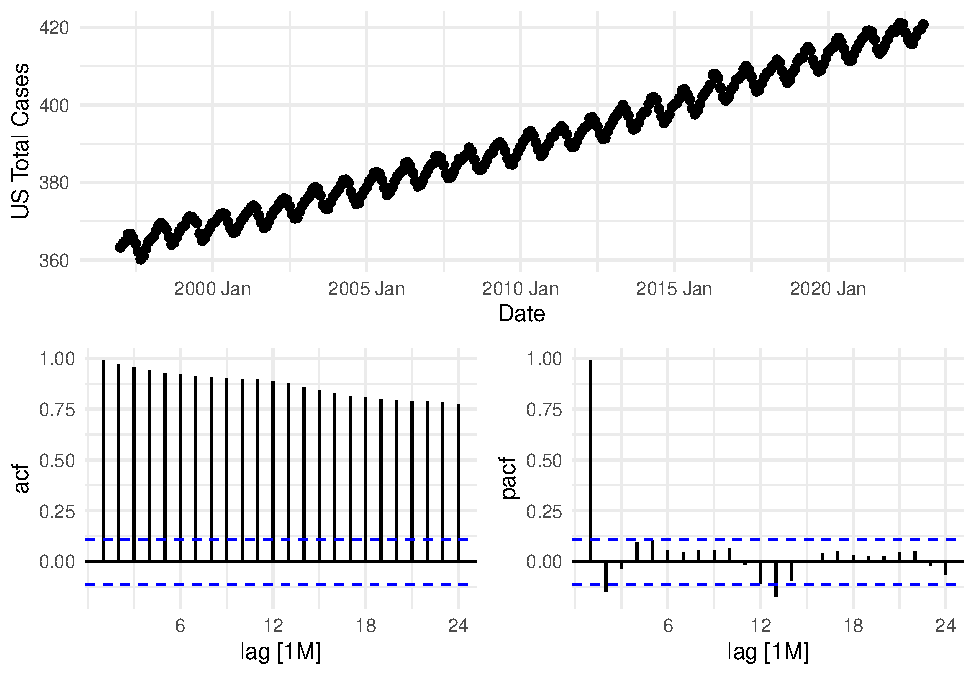
\includegraphics{Lab2_Group_report_files/figure-latex/unnamed-chunk-15-1.pdf}

\hypertarget{points-task-5b-train-best-models-on-present-data}{%
\subsection{(4 points) Task 5b: Train best models on present
data}\label{points-task-5b-train-best-models-on-present-data}}

Seasonally adjust the weekly NOAA data, and split both
seasonally-adjusted (SA) and non-seasonally-adjusted (NSA) series into
training and test sets, using the last two years of observations as the
test sets. For both SA and NSA series, fit ARIMA models using all
appropriate steps. Measure and discuss how your models perform in-sample
and (psuedo-) out-of-sample, comparing candidate models and explaining
your choice. In addition, fit a polynomial time-trend model to the
seasonally-adjusted series and compare its performance to that of your
ARIMA model.

\hypertarget{points-task-part-6b-how-bad-could-it-get}{%
\subsection{(3 points) Task Part 6b: How bad could it
get?}\label{points-task-part-6b-how-bad-could-it-get}}

With the non-seasonally adjusted data series, generate predictions for
when atmospheric CO2 is expected to be at 420 ppm and 500 ppm levels for
the first and final times (consider prediction intervals as well as
point estimates in your answer). Generate a prediction for atmospheric
CO2 levels in the year 2122. How confident are you that these will be
accurate predictions?

\hypertarget{conclusions}{%
\section{Conclusions}\label{conclusions}}

What to conclude is unclear.

While the most plausible model that we estimate is reported in the main,
``Modeling'' section, in this appendix to the article we examine
alternative models. Here, our intent is to provide a skeptic that does
not accept our assessment of this model as an ARIMA of order (1,2,3) an
understanding of model forecasts under alternative scenarios.


\end{document}
